\chapter{Methodology}\label{methodology}
In this section, we are going to discuss the proposed framework and its main components in detail. The proposed method is efficient and computationally inexpensive compared to other methods proposed in literature.

%-------------------------------------------------------------------------
\section{Overview}
\begin{figure}
	\centering
	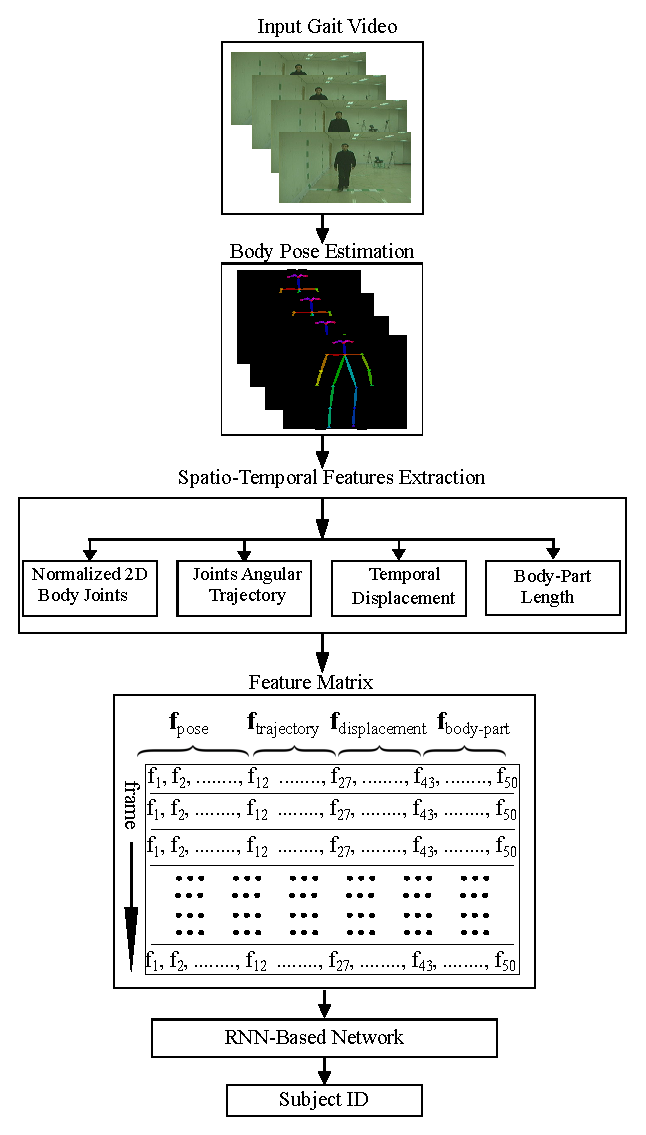
\includegraphics[width=115mm]{figures/proposed_method.eps}
	\caption{
The overview of the proposed framework for gait recognition. 2D human poses were first extracted from raw video frames using improved OpenPose~\cite{Cao_19} algorithm. Effective body joints were then selected from each subject pose estimation and a timestep of 28 frame pose sequence was formed to feed into a temporal network. The temporal network identified the subject by modeling the gait features.
	}
	\label{fig:proposed_method}
\end{figure}

The workflow of our proposed network is illustrated in Figure~\ref{fig:proposed_method} Many strategies have been taken to design and train the network for robust recognition. Firstly, we designed a novel spatio-temporal gait feature descriptors based on the 2D human poses estimated from raw video frames using an improved OpenPose~\cite{Cao_19} algorithm. Thereafter, the gait descriptors were fed into a 2-layer BiGRU network which models the descriptors to recognize the subject ID.


%-------------------------------------------------------------------------
\section{Forming Spatio-Temporal Features}

\subsection{2D Body Joints Feature}
As every joint of the human body does not have a significant role in gait pattern, they cannot improve gait recognition accuracy. Some joints perform even worse. So, among the 25 body joints estimated from OpenPose algorithm we searched out those joints which have a rich and discriminative gait representation capacity. Cunado \textit{et al.}~\cite{Cunado_97} used the human leg-based model as they found that change of human leg contains the most important features for gait recognition.  In our study, we found that knee along with the joints located in feet show more robustness than any other body joints because they do not change while people are walking in cloths or carrying bags. For example, hip joints get wider in coat than normal condition. Again, in some gait videos, some subjects put their hands into their coat pocket, which they cannot do in normal walking. This situation significantly changes the joint coordinates. Hence, we do not consider hip or any other body joints above it.

\begin{figure}
	\centering 
	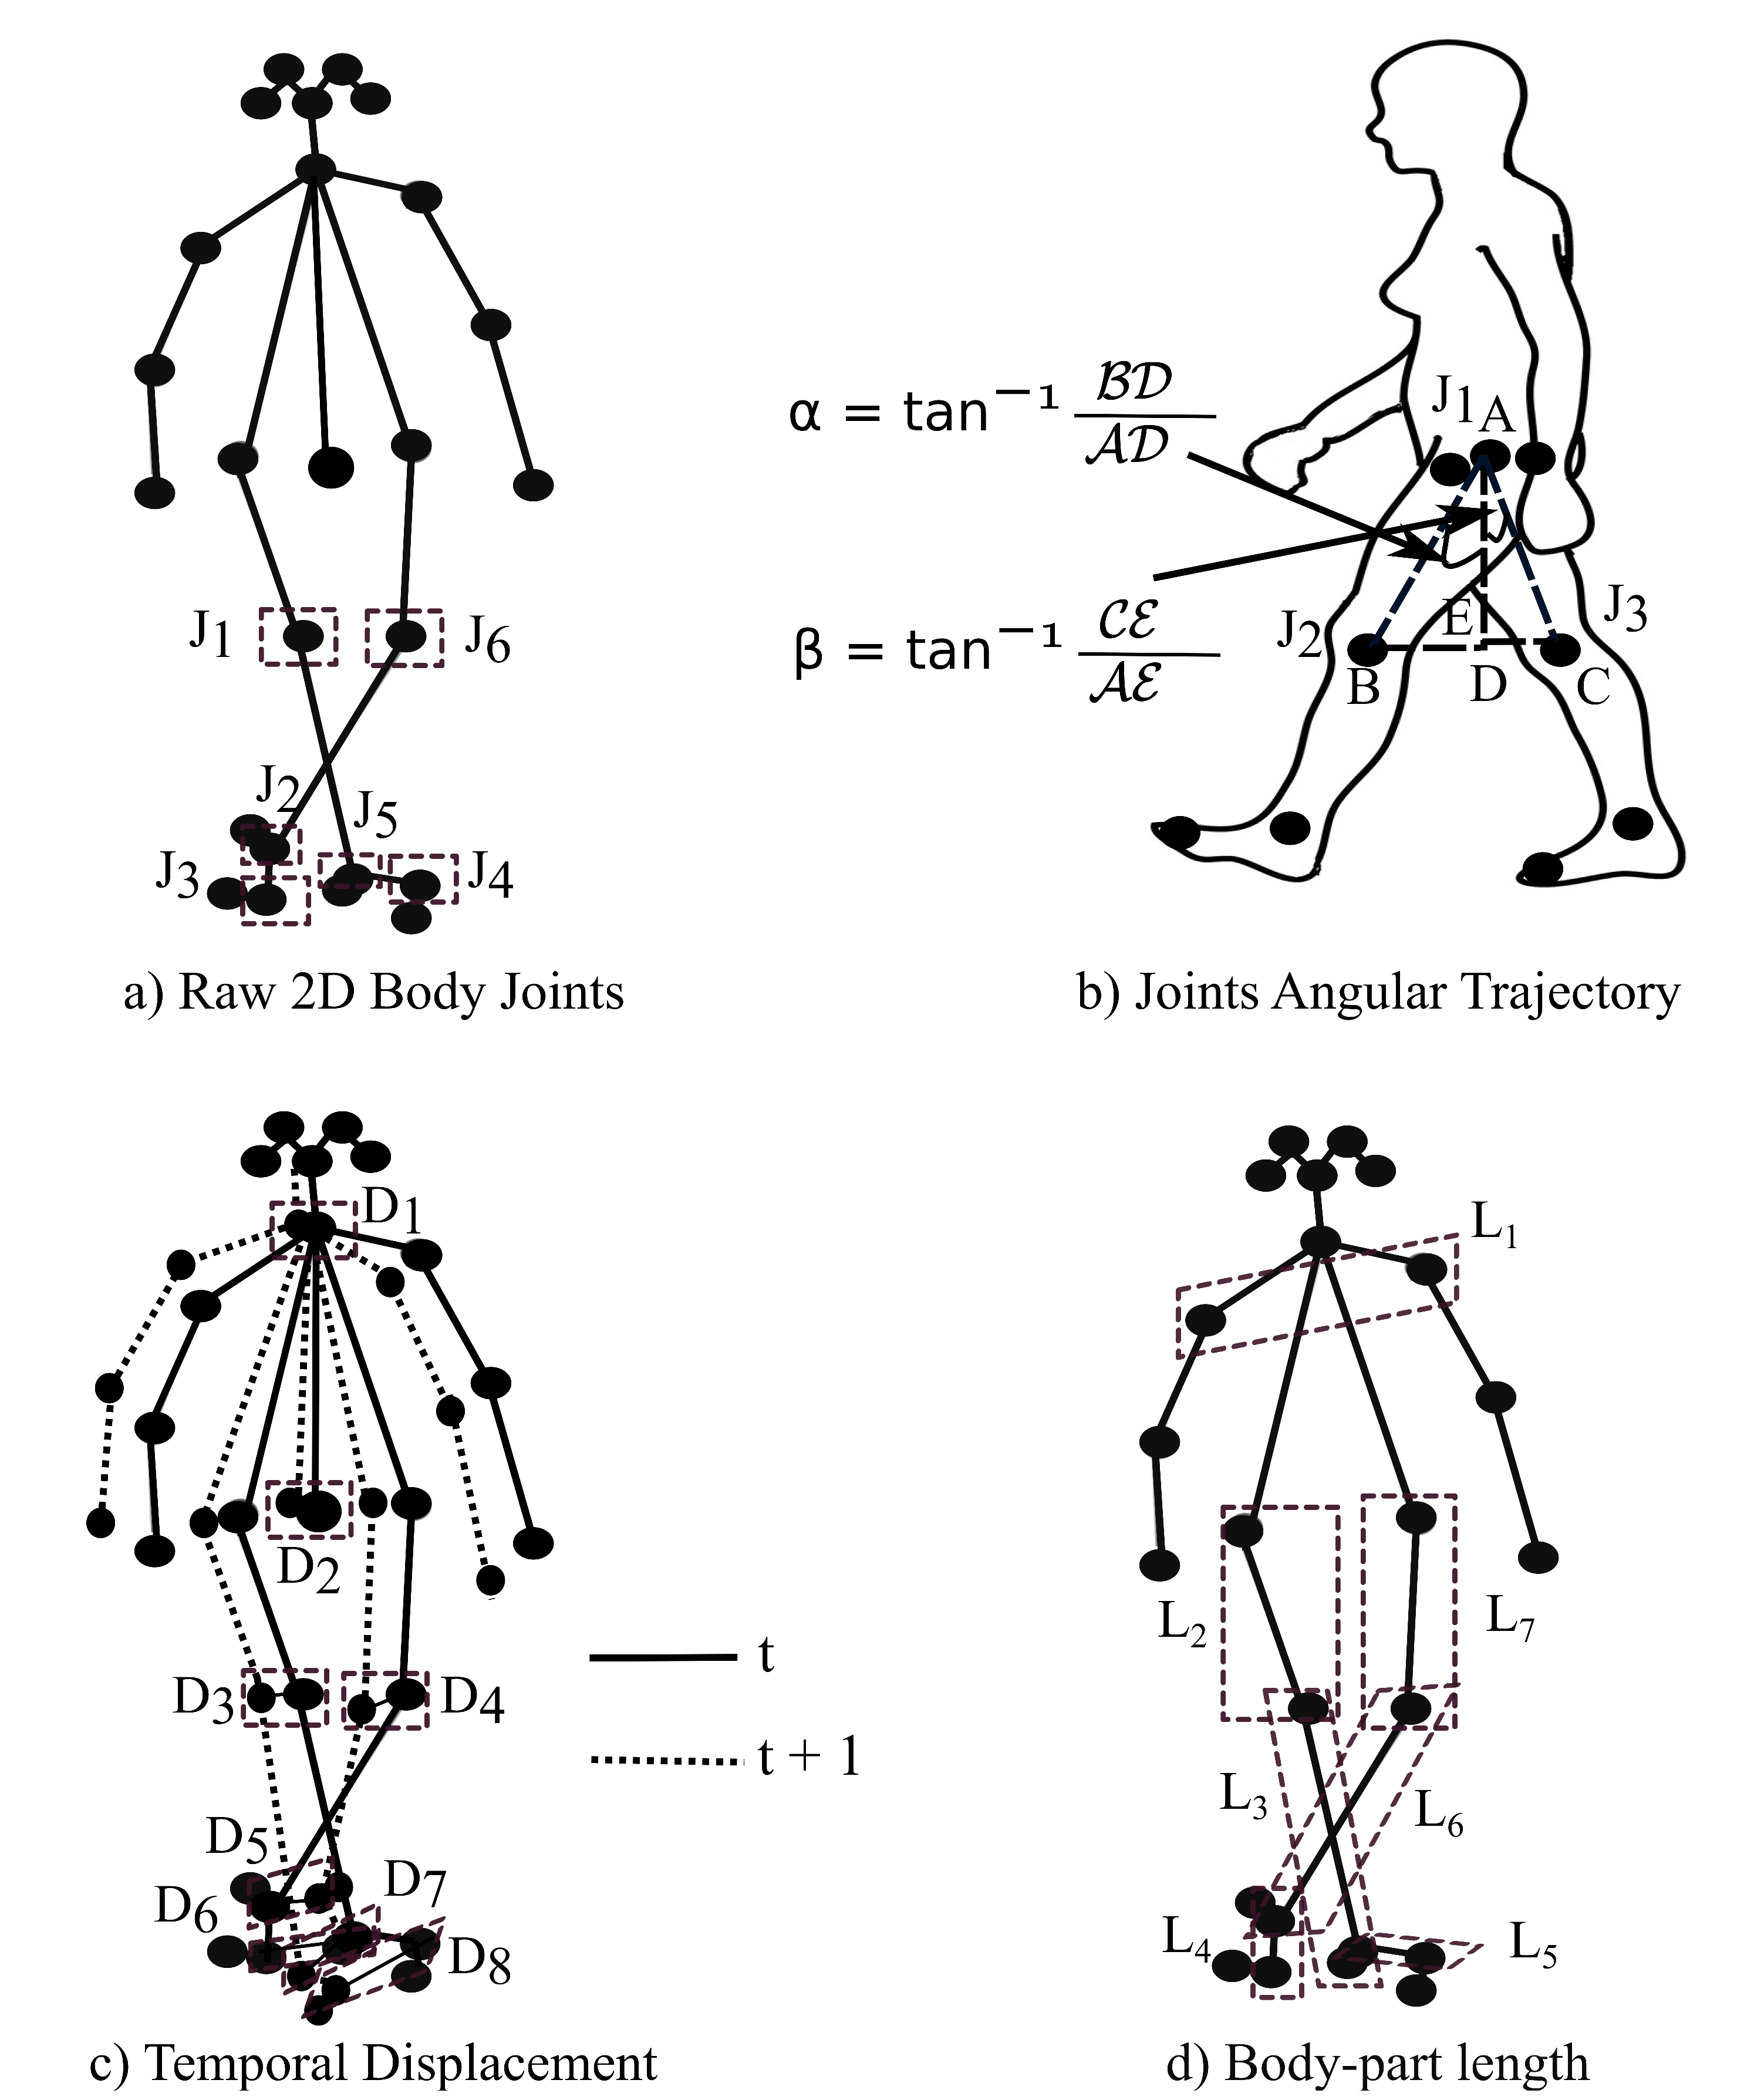
\includegraphics[width = 120mm]{figures/extracted_features.eps}
	\caption{
	Different features extraction process of the proposed method. a) 6 effective joints were selected out of 25 body joints as estimated from pose estimation algorithm~\cite{Cao_19} to form a 12-dimensional pose vector. b) 5 angular trajectories from lower limbs were considered to form a joint-angle feature vector. c) A total of 8 body joints were selected to get temporal displacement features. d) 7 body parts were taken to form a limb length feature vector.
	}
	\label{fig:extracted_features}
\end{figure}

Consequently, in our work, as shown in Figure~\ref{fig:extracted_features}(a) we selected 6 body joints (RKnee, Rankle, RBigToe, LKnee, LAnkle, LBigToe) to form our effective pose features. Thus, we have 12-dimensional pose feature vector, $\textbf{f}_{pose}$, for a single frame. 

\begin{equation}
  \textbf {f}_{pose}= [x_1, y_1, x_2, y_2, \ldots\ldots, x_6, y_6]^T
\end{equation}

It is necessary to normalize the pose sequence data with regard to the subject position in frame, size, or speed of walking to get improved performance. In different gait datasets, as people walk through the fixed camera, the size of the subject’s body changes due to change in the distance between the subject and the camera changes. In our study, to find the origin of the coordinate system ($J_c$) for each subject, we took right, left, and middle of the hip joints and calculated the average of them. Again, to normalize the bodies of different subjects to a fixed size, we took $ h $, the euclidean distance from hip to neck joint, as unit length. 

\begin{equation}
\begin{split}
	Jc &= {(J_{LHip}+J_{RHip}+J_{MHip})} / {3} \\
	h &= \parallel {J_c} – {J_{neck}}\parallel_2  \\
	J_{i}^{N}  &= (J_i – J_c) / h 
\end{split}
\end{equation}
Here, ${J_i}^N$ be the new coordinate of $J_{i}$.


\subsection{Joints Angular Trajectory}
The dynamics of human gait motion can be expressed by the temporal information of joint angles. Hence, discriminative gait features can be found by considering the change in joint-angle trajectory of the lower limbs~\cite{Wang_04}. Therefore, in this study, we formulated a 15-dimensional joint angle features vector $\boldsymbol{f}_{trajectory}$ by considering five lower limb joint-angle trajectories using the following equations. 
\begin{table}
	\centering
	\caption{List of effective joint-angle trajectories with corresponding body joints set for gait angular feature vector \label{table:list_joint_angle_trajectory}}
	\begin{tabular}{cc}
		\hline
		\textbf{Angular Trajectory} & \textbf{Body Joints Set}\\
		
		\hline
		Hip trajectory &10, 8, 13 \\
		Right knee trajectory  &11, 10, 9 \\
		Left knee trajectory &14, 13, 12 \\
		Right ankle trajectory &22, 11, 10 \\
		Left ankle trajectory &19, 14, 13 \\
		\hline
	\end{tabular}
\end{table}

\begin{equation}
	\begin{split}
	\alpha &= 
	\begin{cases}
	\tan^{-1}{\frac{|J_{2,x}-J_{1,x}|}{|J_{2,y}-J_{1,y}|}} & J_{2y} \neq J_{1,y}\\
	\pi/2 & J_{2,y} = J_{1,y}
	\end{cases} \\ \noalign{\vskip10pt}
	\beta &= 
	\begin{cases}
	\tan^{-1}{\frac{|J_{3,x}-J_{1,x}|}{|J_{3,y}-J_{1,y}|}} & J_{3,y} \neq J_{1,y}\\
	\pi/2 & J_{3,y} = J_{1,y}
	\end{cases} \\ \noalign{\vskip10pt}
	\theta &= \alpha + \beta
	\end{split}
\end{equation}

As shown in Figure~\ref{fig:extracted_features} (b), $J_1, J_2, J_3$ are the joints which form a set of angular trajectory. In this work, we considered five sets of angular trajectories from the lower limb of human body. Table~\ref{table:list_joint_angle_trajectory} demonstrated the selected angular trajectories with their corresponding body joints. For each trajectory, we took $(\theta, \alpha, \beta)$s gait features. 

\begin{equation}
\textbf {f}_{trajectory}= [\theta_1, \alpha_1, \beta_1,\theta_2, \alpha_2, \beta_2,\ldots\ldots, \theta_5, \alpha_5, \beta_5]^T
\end{equation}


\subsection{Temporal Displacement}
Our third extracted features were a simple descriptor that preserves temporal information. It stores the local motion features of gait by keeping the displacement information between the two adjacent frames of the pose sequence. Each joint displacement of a frame was then normalized by the total length of all joints. Let, $ t $ and $ (t + 1) $ are two adjacent frames. The displacement information of the coordinates of any body joint of frame $ t $ would be the normalized difference between the corresponding coordinates. 

\begin{equation}
\begin{split}
\triangle x^{t}_{1} &=\frac{x^{t+1}_{1} - x^{t}_{1}}{\sum_{i=1}^{8}\parallel J^{t+1}_{i} - J^{t}_{i}\parallel_2} \\ 
\triangle y^{t}_{1} &=\frac{y^{t+1}_{1} - y^{t}_{1}}{\sum_{i=1}^{8}\parallel J^{t+1}_{i} - J^{t}_{i}\parallel_2} \\ 
{\bf f}_{displacement} &= [\triangle x_{1}, \triangle y_{1}, \triangle x_{2}, \triangle y_{2} \ldots\ldots, \triangle x_{8}, \triangle y_{8}]^{T}
\end{split}
\end{equation}

Here, $J$ it is the 2D coordinates of the $i_{th}$ body joint at $t_{th}$ frame in the video and $(\triangle x_1^t , \triangle y_1^t )$ is the displacement of the coordinates of first joint at t th frame of the video. As shown in Figure~\ref{fig:extracted_features} (c), we selected 8 joints (Neck, MHip, RKnee, Rankle, RBigToe, LKnee, LAnkle, LBigToe) to get a 16-dimensional $\textbf{f}_{displacement}$ vector.


\subsection{Body Part Length Features}
These static gait parameters, e.g., the length of the body parts calculated from joints position are also important for gait recognition~\cite{Wang_04, Araujo_13}. They form spatial gait features which make them robust against covariate such as carrying and clothing variation. In this work, we took seven body parts (Figure~\ref{fig:extracted_features} (d)) namely length of the two leg, two feet, two thigh and width of the shoulder which formed a 8-dimensional spatial feature vector $\textbf{f}_{body-part}$. 


\subsection{Fusion of Features}
Many research works have applied techniques to fuse multiple features to get improved performance~\cite{Liao_19, Wang_04}.  Different types of fusion methods are proposed in literature such as feature level fusion, representation level fusion, and score level fusion. In feature level fusion, multiple features of the same frame are concatenated before feeding into a final network and in representation level, fusion each feature vector is firstly fed into a network and the resulting global representations are then concatenated to train a final classifier. For score level fusion, each feature vector is separately fed into the final network which predicts a classification score. Then, the scores from multiple classifiers are fused using an arithmetic mean.

In this study, we found that features level fusion has produced better recognition results in contrast to other fusion techniques or individual feature sets. 



%-------------------------------------------------------------------------
\section{Feature Preprocessing}
\begin{figure}
	\label{fig:pose_estimation}
	\centering 
	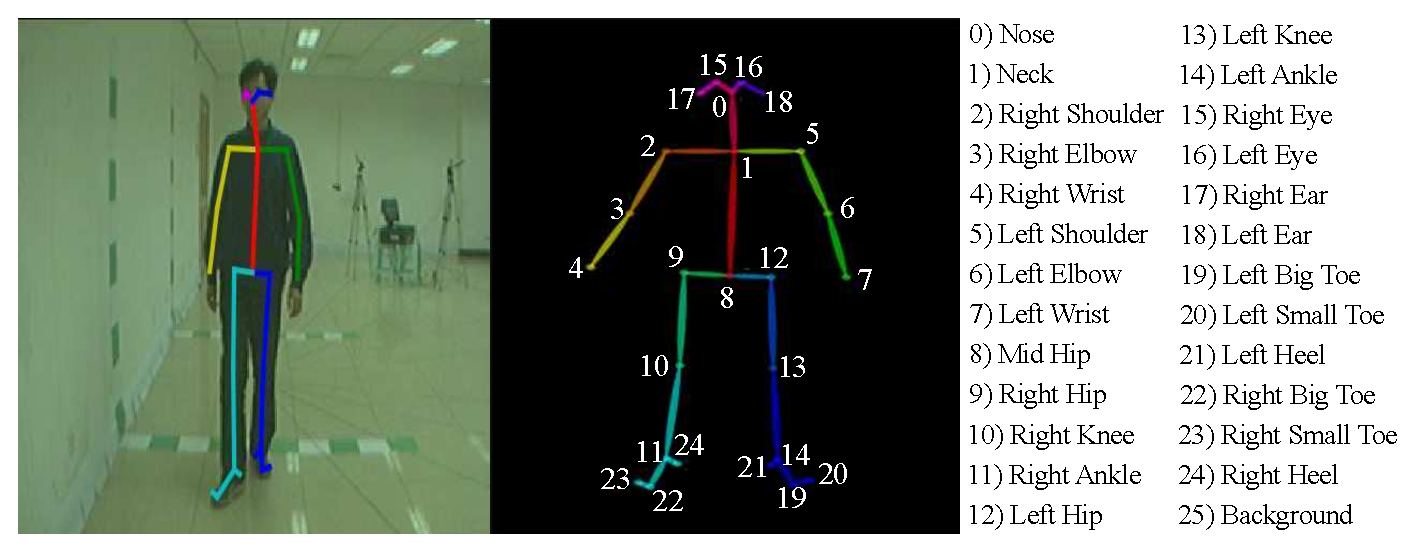
\includegraphics[width = 125mm]{figures/pose_estimation.eps}
	\caption{
		Examples of 2D human pose estimation by~\cite{Cao_19} from RGB images of CASIA dataset (left ones). Detected 25 human body joints with description are shown. (right ones) 
	}
\end{figure}

From 2D pose estimation algorithm~\cite{Cao_19}, we got 25 body joints from each frame (Figure~\ref{fig:pose_estimation}). We took several preprocessing steps to address the problem of missing data due to occlusions. The main strategies are: 
\begin{itemize}
\item If the origin of the coordinate system can't be calculated due to missing hip joints, the frame should be rejected.
\item If more than 1 body joint is missing in between knee and ankle joints of both leg, the frame should be rejected due to having little information.
\item In other cases, individual joints were not located in the frame and a position of $[0.0, 0.0]$  was given to that joint. 
\end{itemize}

The above strategies are simpler which do not require any computation and proven to be effective in addressing the missing data problem. Thus, we designed a 50-dimensional spatial-temporal gait feature vector \textbf{p} from the raw 2D pose estimation of each frame. 

We split a gait video into 28 frames segments. Each 28 frame- segment formed a timestep which can be described by equations (6). Here, \textbf{p} is 50-dimension pose vector for each frame; \textit{\textbf{T}} is the feature matrix for each timestep; N is the total number of timestep sequence, and \textit{\textbf{V}} is the sequence of features for a gait video. 

\begin{equation}
\begin{split}
\boldsymbol{p} &= {[f_1, f_2, f_3, \ldots \ldots, f_{50}]}^T \\
\boldsymbol {T} &= {[\boldsymbol p_1, \boldsymbol p_2, \boldsymbol p_3,  \ldots \ldots, \boldsymbol p_{28}]}^T \\
\boldsymbol V &= {[\boldsymbol T_1, \boldsymbol T_2, \boldsymbol T_3,  \ldots \ldots \boldsymbol T_{N}]}^T \epsilon \quad \mathbb {R}^{28\times 50}
\end{split}
\end{equation}

In CASIA dataset, gait videos of different subject have varying timesteps. The number of timesteps in each gait video depends on the total number of frames where a person is detected. Due to the position of the camera, some angles ${(0^{\circ}, 18^{\circ}, 36^{\circ})}$ have more person detected frame than other angles ${(72^{\circ}, 90^{\circ}, 108^{\circ})}$. Therefore, the total number of timesteps in a gait video is different for different subjects and viewing angles. This eventually makes our train dataset unbalanced. Again, in CASIA B dataset, not all subjects have all gait videos; there are some missing gait videos. To solve the problem, we develop our own balance training set by making each subject pose sequence to have a fixed number timesteps. We first found the subject which had maximum timesteps for a particular gait angle and then augmented other subject's timesteps with that specific length by overlapping their sequences.


\subsection{Data Augmentation}
The performance of deep neural networks is strongly correlated with the amount of available training data.  Although CASIA is the largest gait dataset, the standard experimental setup of this dataset (see Table IV) allows us to train only the four normal walking sequence of each subject. Therefore, we need to augment our train data to obtain a stable model.  
One way to increase the amount of training data is to overlap video clips Therefore, we split the input video into an overlapping sequence of video clips. For every 28 image clip, we overlapped 24 images of the previous clip at almost $ 85.7\% $ overlapping rate. For example, a particular gait video of 100 frames would be split into the clips $(1-28), (5-32), (9-36), ...$ up to frames $(73, 100)$. 

In addition to above technique, we further augment our training data by adding another gait sequence (i.e., $ 25\% $ increment) by implementing Gaussian noise to a given normal walking sequence. 

\begin{equation}
N(j_i) = (x + \tilde{x},  \quad y+ \tilde{y})
\end{equation}

Here,  $\tilde{x}$ and $\tilde{y}$ are two random real numbers generated by a normal distribution with zero mean and unit standard deviation. We apply noising (N) into the raw joints position of a training pose data.



\subsection{Network Architecture}
\begin{figure}
	\centering 
	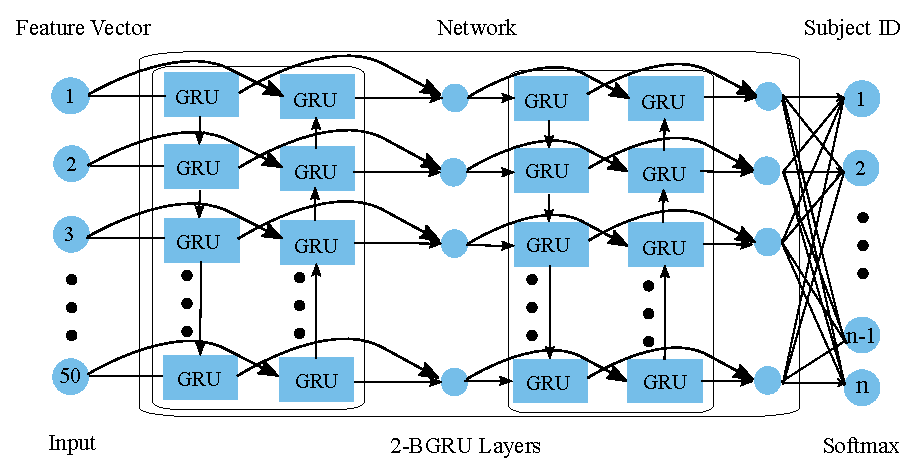
\includegraphics[width = 115mm]{figures/rnn_network.eps}
	\caption{
		Proposed \gls{rnn} architecture for robust gait recognition. It consists of two \gls{bigru}~\cite{Schuster_97} layers each of which consists of 80 \gls{gru} cells with one batch normalization and one output softmax layer. The network was fed with 50 dimensional input from 2D pose estimation. Input layer was followed by a batch normalization layer~\cite{Ioffe_15}. The output of recurrent layers was also batch normalized to standardize the activations and finally fed into an output softmax layer. For the output layer, the number of the output neuron equals to the number of subjects.
	}
	\label{fig:rnn_network}
\end{figure}
In this research, we experimented with different \gls{rnn} architectures such as Gated Recurrent Units (\gls{gru}s),  Long Short-Term Memory Units (\gls{lstm}s), Bidirectional Long Short-Term Memory (\gls{bilstm}) and Bidirectional Gated Recurrent Units (\gls{bigru})~\cite{Schuster_97}. Firstly, we designed the proposed network employing all these architectures with one recurrent layer and then, searched for optimum recurrent unit size between 50 to 150. Thereafter, we increased the capacity of the network by adding the second and third layers of hidden units. Finally, we found that, among different RNN-based architectures, 2-layer BiGRU with 80 hidden units performs best. 

After input and the second recurrent layer, we placed a batch normalization (\gls{bn})~\cite{Ioffe_15} layer. At last, a fully connected layer with softmax activation was used to output the subject classes. Figure~\ref{fig:rnn_network} illustrates the architecture of the proposed network. 


\subsection{Training}
The training of \gls{rnn}s allows us to learn the parameters from the sequence. We have employed Adam~\cite{Kingma_15} optimization algorithm with $\beta_1 = 0.9, \beta_2 = 0.999$, which is known to work very well for training recurrent neural networks. We tried several learning rates in our experiment and found out that the best initial learning rate is $(1$x$10^{-3})$. We also reduced the learning rate by a factor when it hit a plateau. Reducing the learning rate will allow the optimizer to get rid of the plateaus in loss surface. Table~\ref{table:summary_tn} summarizes all the hyperparameters settings of our network.

\begin{table}
	\centering
	\caption{Training summary of our proposed temporal network. \label{table:summary_tn}}
	\begin{tabular*}{32pc}{@{\extracolsep{\fill}}ll@{}}
			\hline \noalign{\vspace{3pt}}
			\textbf{Hyperparameter} &\qquad \textbf{Value} \\ [3pt] \hline\noalign{\vspace{3pt}}
			Optimizer     			&\qquad Adam~\cite{Kingma_15} \\[3pt]
			Objective function  	&\qquad Fusion of softmax and center loss \\[3pt]
			Epochs        			&\qquad $ 450 $ \\ [3pt]
			Initial learning rate	&\qquad $5 \times 10^{-3}$  \\[3pt]
			Mini-batch size			&\qquad $ 256 $ \\
			\hline
	\end{tabular*}
\end{table}

Our network was trained with a 256 batch size and 28 image clips with one timestep. Our network showed some overfitting mostly due to the high learning capacity of the network over data. This overfitting problem has been addressed by adding a batch normalization layer. 

We also tried to add dropout layer during training, but that did not help to reduce the overfitting problem. Moreover, it degraded gait recognition performance. Hence, we skip it.


\subsection{Loss functions}
In this work, we found that due to the influence of various covariate factors, intraclass distance related to one subject is sometimes more significant than interclass distance. Now, if we only use the \textit{cross-entropy loss} (\gls{ce}) as our objective function, the resulting learned features may contain large intraclass variations. Therefore, to effectively reduce the intraclass distance, we used \textit{center loss} (\gls{cl}), introduced by Wen \textit{et al.}~\cite{Wen_16} for face recognition task. As the training progresses, the center loss learns a center for features of each class and the distances between the features and their corresponding class centers are minimized simultaneously. However, using only center loss may lead the learned features and centers close to zeros due to the very small value of the center loss. Hence, with the fusion of softmax loss ($L_s$) and center loss ($L_c$), we can achieve discriminative feature learning by increasing interclass dispersion and compacting intraclass distance as much as possible.


\begin{equation}
\label{equ:equ_4}
\begin{split}
L_s &=-\sum_{i=1}^{m}log{\frac{e^{W_{y_i}^{T}x_i + b_{y_i}}}{\sum_{j=1}^{n}{e^{W_{j}^{T}x_i+ b_j}}}} \\
L_c &= \frac{1}{2}\sum_{i=1}^{m}{\parallel{{\boldsymbol x_i}-{\boldsymbol c_{y_i}}}\parallel}_2^2 \\
L &= L_s + \lambda L_c + \lambda_{\theta}\parallel{\theta}\parallel_{2}
\end{split} 
\end{equation}

Equations~(\ref{equ:equ_4}) describes total loss ($ L $) calculation of our network. where $\boldsymbol x_{i} \epsilon \mathbb {R}^d$ denotes the $i$th pose sequence which belongs to the $y_i$th class and  $\boldsymbol c_{y_i} \epsilon \mathbb {R}^d$ denotes to the $y_i$th class center of the learned pose features. $W \epsilon \mathbb {R}^{d\times n}$ is the feature dimension of the last fully connected layer and $b\epsilon \mathbb {R}$ is the bias term of the network. The batch size and the class number are m and n respectively. $\lambda$, a scalar variable, is set to value 0.01 to balance the two loss functions. $\parallel{\theta}\parallel_{2}$ refers to the kernel regularizer for all the parameters of the network with a weight decay coefficient $(\lambda_{\theta})$ set to $0.0005$ for the experiment.  


\subsection{Post-processing}\label{sec_3.1.8}
While training, our proposed temporal network considers each of these video clips as a separate video (see Fig.~\ref{fig:output_prediction}). For a given video, the prediction of our model is a sequence of class probabilities for each of the timestep, i.e. 28 frame clips.
\begin{figure}
	\centering
	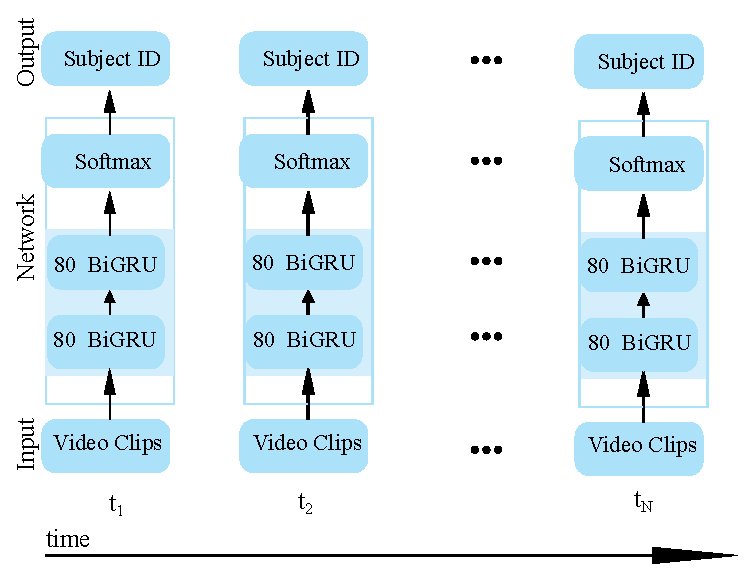
\includegraphics[width = 105mm]{figures/output_prediction.eps}
	\caption{
		Output prediction scheme of our proposed temporal network. Each input clip was considered as a separate video and a sequence of class probabilities was predicted at output. Majority voting scheme was used to process the output to predict the subject ID.
	}
	\label{fig:output_prediction}
\end{figure}

But, while testing, we actually need the subject ID of the complete gait video. Therefore, we used (\textit {majority voting scheme}) to process this output to predict the subject ID. In this scheme, the subject that receives the highest number of votes over all timesteps of a particular gait video is referred as the predicted class.

Let\rq s consider, $\boldsymbol{s}$ is a vector of $n$ number of subjects. For a particular timestep $t$ of a gait video, input pose sequence vector $\boldsymbol X^t \epsilon \mathbb {R}^{28\times 50}$ has an n-dimensional output vector $\boldsymbol o^t$.
\begin{equation}
\begin{split}
\boldsymbol s^t &=  {[s_1, s_2, s_3, ....., s_{n}]}^{T}\\
\boldsymbol o^t &=  {[o_1, o_2, o_3, ....., o_{n}]}^{T}
\label{equ:equ_5}
\end{split}
\end{equation}

Here, $o_i^t = P(s_i | X^t)$ refers the probability of input pose vector $\boldsymbol X^t$ belongs to class $s_i$. Now, we assign the output class $s^t$ to the subject class $s_i$ which have maximum probabilities for the timestep $t$. As each of our gait videos is divided into a series of timestep sequence (see equation~\ref{equ:equ_2}), using majority voting scheme we can have the subject ID. Following equations described the voting scheme.

\begin{equation}
\begin{split}
s_t &=  \arg\max_{s_i}{\{o_i^t | 1 \leq i \leq n\}} \\
s &= {\arg\max}_{i\in(1, 2, ...,n)}{\sum_{t=1}^{N}s_i^N}
\end{split}
\end{equation}
Here, N is the total number of timesteps in which a gait is split and s is the final predicted class.  


%-------------------------------------------------------------------------
\section{Multi-View gait recognition}
\begin{figure}[t]
	\centering
	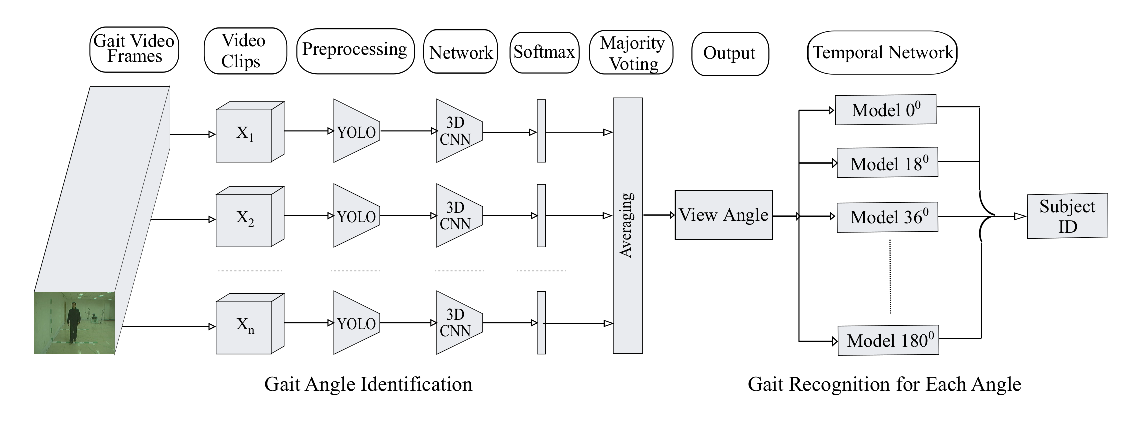
\includegraphics[width=130mm]{figures/multi_view_gait_recognition.eps}
	\caption{
		Overview of our proposed multi-view gait recognition network scheme. YOLOv3~\cite{Redmon_18} was used to detect and locate the walking people in video frames. The input of the network was a clip of 16 consecutive frame which was preprocessed and resized to $112\times112$ to feed into a 3D convolutional network based on C3D~\cite{Tran_15}. The network used 3D kernels to exploit spatio-temporal dynamics for viewing angle identification. Thereafter, a temporal network, trained on each viewing angle, was performed subject identification by modeling temporal dynamics from input 2D pose sequence
	}
	\label{fig:multi_view_gait_recognition}
\end{figure}

The workflow of our proposed two-stage multi-view gait recognition network is illustrated in Fig.~\ref{fig:multi_view_gait_recognition}. In first stage, we trained a 3D convolutional network to estimate the walking direction of the subject by extracting spatio-temporal features from gait video. Thereafter, we performed subject recognition using proposed temporal network which has been trained for that particular angle.

%-------------------------------------------------------------------------
\subsection{Preprocessing}
Firstly, to localize human walking in gait videos, we used YOLOv3, a state-of-the-art real-time object detection algorithm, proposed by Redmon \textit{et al.}~\cite{Redmon_18}. We then cropped each of the person detected frame using the bounding box coordinates found from YOLOv3 algorithm and resized them to $112\times112$ for our network input. Thereafter, we splitted each gait video into overlapping sequences of 16 consecutive frames within training or test set. There is an overlap of 8 frames (50\%) indicating that the samples were gathered using a 16 frame sliding window with a 50\% stride.


%-------------------------------------------------------------------------
\subsection{Network architecture}
Identifying walking direction from gait video is somewhat similar to action recognition problem in computer vision. Recently, in action recognition, researcher have started to exploit 3D features in video using 3D-CNN model which extracts features from both spatial and temporal dimensions by performing 3D convolutions. Tran et.al.~\cite{Tran_15} proposed a 3D convolutional neural network, also known as C3D, which has been widely used for applications like video classification, action recognition, etc. This network has been trained on one of the largest video classification benchmark datasets Sports-1M~\cite{Karpathy_14}. The dataset contains 1.1 million sports videos, where each video belongs to one of the 487 sports categories. 

The proposed method for our gait angle identification is illustrated in Fig.~\ref{fig:multi_view_gait_recognition}. The input of the network was a clip of 16 consecutive frame which was preprocessed and resized to $112\times112$ to feed into a a 3D-CNN network. We used {\textit {majority voting scheme}} to process the output to predict the view angle similar to section~\ref{sec_3.1.8}, i.e. the angle that receives the highest number of votes over all clips are referred as predicted angle of the video.

\begin{figure}
	\centering {
\includegraphics[width=140mm]{figures/3D_CNN.eps}}
	\caption{
		Proposed 3D-CNN for video angle identification. Last 3 layers of a pretrained C3D~\cite{Tran_15} network has been replaced by a fully connected layer of 128 neurons followed a final softmax layer of 11 neurons to classify 11 different walking direction in CASIA-B dataset.
	}
	\label{fig:3D_CNN}
\end{figure}

\begin{table}
	\centering
	\caption{Training summary of our proposed 3D-CNN network.  \label{table:summary_3dcnn}}
	\begin{tabular*}{30pc}{@{\extracolsep{\fill}}ll@{}}
			\hline \noalign{\vspace{3pt}}
			\textbf{Hyperparameter} & \textbf{Value} \\ \hline\noalign{\vspace{3pt}}
			Optimizer  &Stochastic gradient descent (\gls{sgd})  \\ [3pt]
			Objective function  &Mean squared error (\gls{mse}) \\ [3pt]
			Epochs  &70  \\ [3pt]
			Initial learning rate & $1 \times 10^{-3}$ \\ [3pt]
			Mini-batch size	  &12  \\ [3pt]
			Momentum  &0.92 \\ [3pt]
			\hline
	\end{tabular*}
\end{table}

Successful transfer learning within or across different domain of interest leads to significant improvement in performance due to the amount of jointly learning representations in a shared feature space. In our work, we used a pretrained C3D model and fine-tuned it for our 3D Convolutional network to determine the viewpoint angle from gait videos. Fig.~\ref{fig:3D_CNN} shows our proposed 3D convolutional network. 

C3D network is composed of 8 convolutional layers, 5 pooling layers, 2 fully-connected layers, followed by a softmax layer at the end. All the 3D convolution kernels are $3\times3\times3$ with stride 1 in both spatial and temporal dimensions. We removed the last 3 layer from the model and then added a fully connected layer of 128 neurons and a dropout layer of 0.5 to avoid overfitting. Finally, a softmax layer of 11 neuron has been added to classify any given videos into 11 different viewing angles. 


%-------------------------------------------------------------------------
\subsection{Training}
We used CASIA-B gait dataset~\cite{Yu_06} to train our model. We trained the network using 4 normal walking sequences of 100 subject in gallery set of CASIA-B as described in Table~\ref{table:caisab_setup}. Our network was trained with a 12 batch size with an initial learning rate ${10^{-3}}$ for 70 epochs. Table~\ref{table:summary_3dcnn} summarizes all hyper-parameters setting of our proposed network.

\endinput